\section{Spørgsmål 2}

\subsection{Fokuspunkter}
\begin{itemize}
	\item Hvorledes omsættes et konceptuelt databasedesign til en konkret database?
	\item Kom bla. ind på begreberne "\textit{designregler}, \textit{relations modellering}, samt \textit{skema}.
\end{itemize}

\subsection{Litteratur}
\begin{itemize}
	\item Kap. 2 fra \textit{Database eLearning} - $http://db.grussell.org/index.html)$
	\begin{itemize}
		\item Database Analysis.
		\item Entity Relationship Modelling.
		\item Mapping ER Models into relations.
		\item Advanced ER Mapping.
	\end{itemize}
	\item Database Modelling and Design
	\begin{itemize}
		\item Kap. 1 (s. 1 - 11).
		\item Kap. 3 (s. 35 - 53).
		\item Kap. 5 (s. 85 - 108).
	\end{itemize}
\end{itemize}

\newpage

% must
\subsection{Hvorledes omsættes et konceptuelt databasedesign til en konkret database?}
Som i objektorientering: finder
betydende klasser i problemdomænet. Analyserer klassernes association, baggrund af disse opstilles en model for den kommende database. Modellen er typisk udført i et Entity Relationship Diagram (ER) eller i et klassediagram (UML).

\begin{enumerate}
	\item Identificer entiteter og deres attributter.
	\item Definer relationer mellem entiteterne.
	\item Anvend De 10 designregler.
\end{enumerate}

En grund til at lave et velovervejet design er at minimere risikoen for anormaliteter, dvs. fejl eller uregelmæssigheder der opstår i data. Her kan også anvendes normalisering (se side~\pageref{sec:normal}).

\subsubsection{Faldgruber}
Når designet laves, er der faldgrupper. Det kan f.eks. være en \textbf{fan trap} eller \textbf{chasm trap}. Disse er kendt som \textbf{Connection Traps} 

\paragraph{Fan trap} opstår, når en entitet har \textit{1:M} relation til mindst to entiteter. Hvilket betyder at ''vejen'' fra \textit{Dept.} til \textit{Staff} bliver tvetydig. 

På figur~\ref{fig:fan} kan man se at et \textit{Site} har flere \textit{Department} og \textit{Staff}. Problemet bliver så: \textit{''which staff work in a particular department?''}

\begin{figure}[h]
\centering
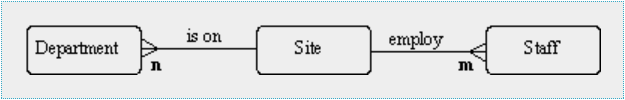
\includegraphics[width=0.8\linewidth]{figs/spm2/fan}
\caption{Fan Trap.}
\label{fig:fan}
\end{figure}

På figur~\ref{fig:fan_solved} vises det hvordan problemet løses ved at ændre ER modellen til at vise den korrekte association.

\begin{figure}[h]
\centering
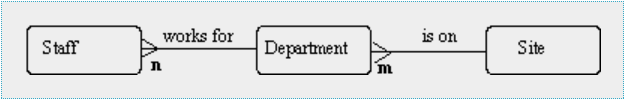
\includegraphics[width=0.8\linewidth]{figs/spm2/fan_solved}
\caption{Fan Trap Resolved.}
\label{fig:fan_solved}
\end{figure}

\paragraph{Chasm trap} 

Finder sted når der bør være en relation mellem to entities, men 'stien' imellem dem findes ikke for nogle forekomster. På figur~\ref{fig:chasm} ses problemet.

\begin{figure}[H]
\centering
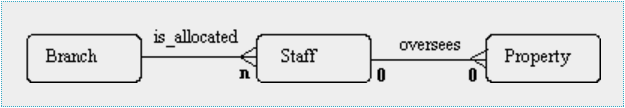
\includegraphics[width=0.75\linewidth]{figs/spm2/chasm}
\caption{Chasm trap.}
\label{fig:chasm}
\end{figure}

\textit{Branch} har indirekte en relation til \textit{Property}, men da \textit{Property} ikke skal være tilknyttet en \textit{Staff} opstår problemet. For nu kan \textit{Branch} ikke finde 'ned' til \textit{Property}.

På figur~\ref{fig:chasm_solved} ses løsningen, hvor der simpelthen er lavet en relation til \textit{Property} fra \textit{Branch}.

\begin{figure}[H]
\centering
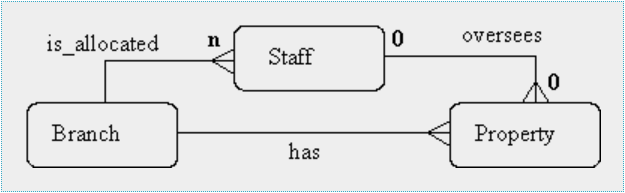
\includegraphics[width=0.7\linewidth]{figs/spm2/chasm_solved}
\caption{Chasm trap resolved.}
\label{fig:chasm_solved}
\end{figure}


% must
\subsection{De 10 Designregler}

\begin{enumerate}
	\item \textbf{Entity}
	\begin{itemize}
		\item Én entitet skal svare en én tabel. Entiteten skal have samme navn som tabellen.
	\end{itemize}
	
	\item \textbf{Many-to-many binary relationship}
	\begin{itemize}
		\item Entiteternes primærnøgler bliver sammensat i en ny entitet hvor de er fremmednøgler, kaldet en \textit{weak entity\footnote{Pga. manglende primærnøgle.}}.
	\end{itemize}
	
	\item \textbf{One-to-many binary relationship}
	\begin{itemize}
		\item ''Mange''-entiteten skal have en fremmednøglen, som peger på 'en'-entititens primærnøgle. Ellers brydes 1. normalform.
	\end{itemize}
			
	\item \textbf{Recursive binary relationship}
	\begin{itemize}
		\item Samme regler er gældende som ved øvrige binære relationer.
	\end{itemize}
	
	\item \textbf{Ternary relationship}
	\begin{itemize}
		\item En weak-tabel oprettes med en primær nøgle der er sammensat af de 3 fremmednøgler.\todo{Sammensat? Composite nøgle?}
	\end{itemize}
	
	\item \textbf{Attribute of an entity}
	\begin{itemize}
		\item En attribut af en entitet skal mappes direkte som en attribut i entitetens tabel.
	\end{itemize}
	
	\item \textbf{Generalization super-class (super-type) entity}
	\begin{itemize}
		\item En super entitet mappes direkte til en SQL tabel.
	\end{itemize}
	
	\item \textbf{Generalization sub-class (subtype) entity}
	%En sub entitet mappes til sin egen table for super entiteten. Primær nøglen fra super entiteten	bliver fremmednøgle hos sub entiteten.
	\begin{itemize}
		\item Skal mappes direkte til SQL, men med superklassens primærnøgle som en fremmednøgle.
	\end{itemize}
	
	\item \textbf{Mandatory constraint on the 'one' side of a \textit{1:M relationship}}
	\begin{itemize}
		\item 'En'-entiteten af et \textit{1:M} relation skal altid være mandatory.
		\item Fremmednøglen i 'mange'-entiteten skal være 'NOT NULL'.
	\end{itemize}
		
	\item \textbf{Subject gets targets Primary key as foreign key}
	\begin{itemize}
		\item Bruges ved \textit{1:1} relationer hvis de opstår.
		\item Identificerer target (den som har interesse i subjekt).
		\item Subjekt får targets primærnøgle som fremmednøgle.
		\item Hvis en af entiteterne er mandatory skal den have primærnøglen.
	\end{itemize}
	
\end{enumerate}

% must
\subsection{Relationsmodellering}

% must
\subsection{Skema}
Et skema er det DDL\footnote{Database Definition Language}, der beskriver strukturen i databasen.
Strukturen består af:

\begin{itemize}
	\item Tabeller i databasen.
	\item Attributter i tabellerne.
	\item Hvilke attributter, der bruges som keys.
	\item Hvor fremmednøgler peger hen.
	\item Hvilke attributter, der udgår composite keys (se side~\pageref{sec:keys}).
\end{itemize}





























